\section*{Results}


With two traits, trait evolution followed patterns associated with the type 
of tradeoff the two traits had when evolved together
(i.e., with the value of $\eta$)
(Figure \ref{fig:two-trait-outcomes}).
When the tradeoff is sub-additive ($\eta = -0.6$), there is a single
stable point in the trait space, where both traits are
maximized---within the limits imposed by traits' negative effects on 
the growth rate.
When the tradeoff is super-additive ($\eta = 0.6$), there are two
alternative stable states, one for each trait being maximized while the 
other is zero.
Lastly, when the tradeoff is additive ($\eta = 0$), traits
evolve to any point on a neutrally stable ring.
The locations of these states are determined by 
the baseline growth rate, 
the cost of increasing traits on the growth rate,
and, when $\eta \ne 0$, the non-additive tradeoff
(Equations \ref{eq:two-traits-finals-eta-negative},
\ref{eq:two-traits-finals-eta-zero}, and 
\ref{eq:two-traits-finals-eta-positive} for 
$\eta < 0$, $\eta = 0$, and $\eta > 0$, respectively).

\begin{figure}[ht!]
\centering
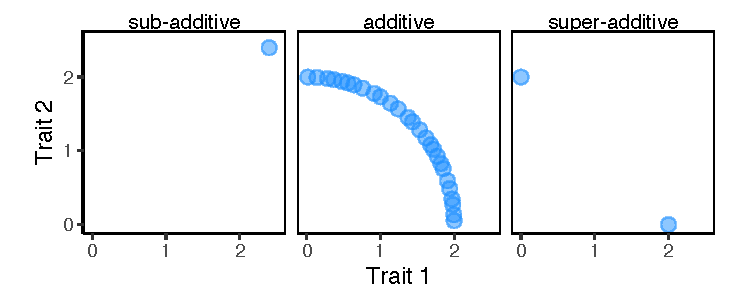
\includegraphics{1-outcomes_q2.pdf}
\caption{Unique trait values for surviving species in simulations of 2-trait communities,
    for tradeoffs being sub-additive ($\eta < 0$), additive ($\eta = 0$), or 
    super-additive ($\eta > 0$).}
\label{fig:two-trait-outcomes}
\end{figure}




The proportion of the 100 species introduced to communities that survived and
coexisted depended on the additive genetic variance, 
the non-additive tradeoffs, and 
how conflicting / non-conflicting evolution was (i.e., the values of $d_1$ 
and $d_2$) (Figure \ref{fig:coexistence-spp}A).
Greater additive genetic variance increased the probability of evolutionary 
rescue, where species evolved quickly enough towards a fitness peak to
prevent themselves from going extinct.
Sub-additive tradeoffs resulted in greater numbers of species because
the lower cost of evolving multiple traits caused species to evolve
high values of both traits.
When combined with non-conflicting evolution,
this decreased competition experienced by all species, both on a 
per-capita basis (the term $- \mathbf{V}_{j}^{\text{T}} \mathbf{D} \mathbf{V}_j$ 
in equation \ref{eq:competition})
and overall (because all $N_j$ are greater).
Increasing $d_1$ and $d_2$ caused greater number of species to coexist
because species evolving toward a fitness peak benefited rather than 
harmed other species with high $d_1$ and $d_2$.
There was an abrupt change when evolution was conflicting for both traits 
(i.e., $d_1 < 0$ and $d_2 < 0$),
where only one species ever survived.

When we kept evolution for the first trait non-conflicting ($d_1 = 0.1$) and
adjusted evolution for trait 2, the results were slightly more complicated
(Figure \ref{fig:coexistence-spp}B).
Additive genetic variance had a similar effect as when we varied both traits' evolution.
The effect of varying $d_1$, however, depended on the tradeoffs.
With sub-additive tradeoffs, the threshold for coexistence was $d_1 = -0.1$.
This is because species evolve to maximize both traits, so $d_1 + d_2$
determines the coexistence behavior of the community.
When tradeoffs are super-additive, $\min (d_1, d_2)$ determines whether 
coexistence can occur.
This is because under super-additivity, species evolve to maximize one trait while 
the other evolves to zero.
When one $d$ is negative, if sufficient species are added to the community and 
each starts with random trait values, 
one will inevitably evolve to maximize the trait that is conflicting. 
That species will exclude all others.


\begin{figure}[ht!]
\centering
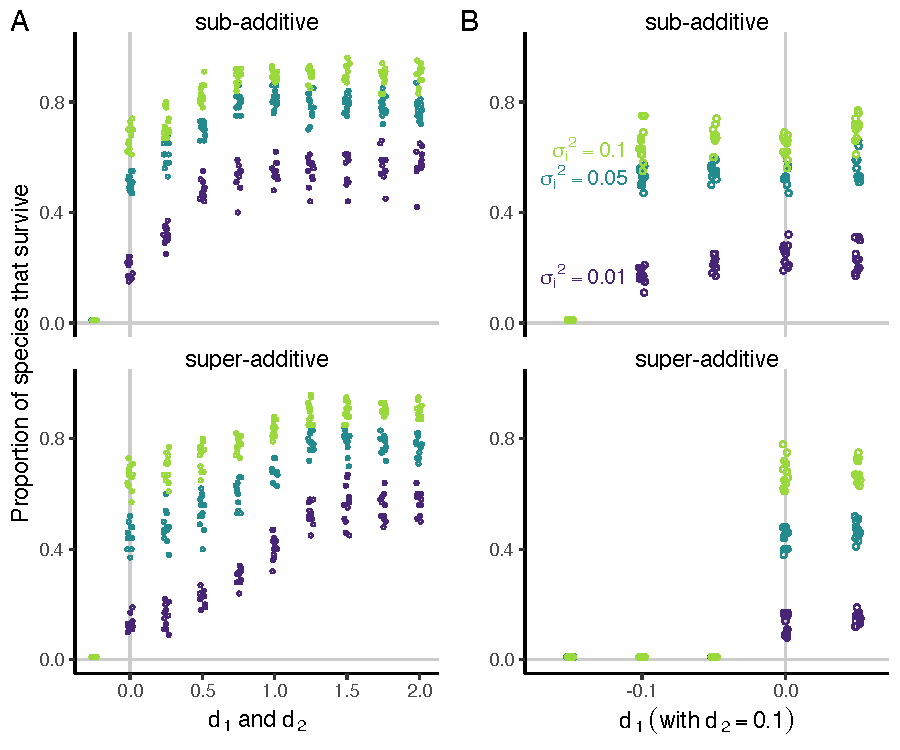
\includegraphics{2-coexist_spp.pdf}
\caption{Proportion of species that survived in simulations of 100-species, 2-trait
    communities with varying additive genetic variances ($\sigma_i^2$), and 
    varying (A) $d_1$ and $d_2$ or (B) varying $d_1$ with $d_2$ fixed at 0.1.
    Shown are both sub-additive ($\eta < 0$) or super-additive ($\eta > 0$) tradeoffs.}
\label{fig:coexistence-spp}
\end{figure}




% ------------------------------------------------------------------------------
% ------------------------------------------------------------------------------
% ------------------------------------------------------------------------------
% ------------------------------------------------------------------------------
% 
% LEFT OFF HERE
% 
% ------------------------------------------------------------------------------
% ------------------------------------------------------------------------------
% ------------------------------------------------------------------------------
% ------------------------------------------------------------------------------



\ref{fig:conditional-coexistence}


\begin{figure}[ht!]
\centering
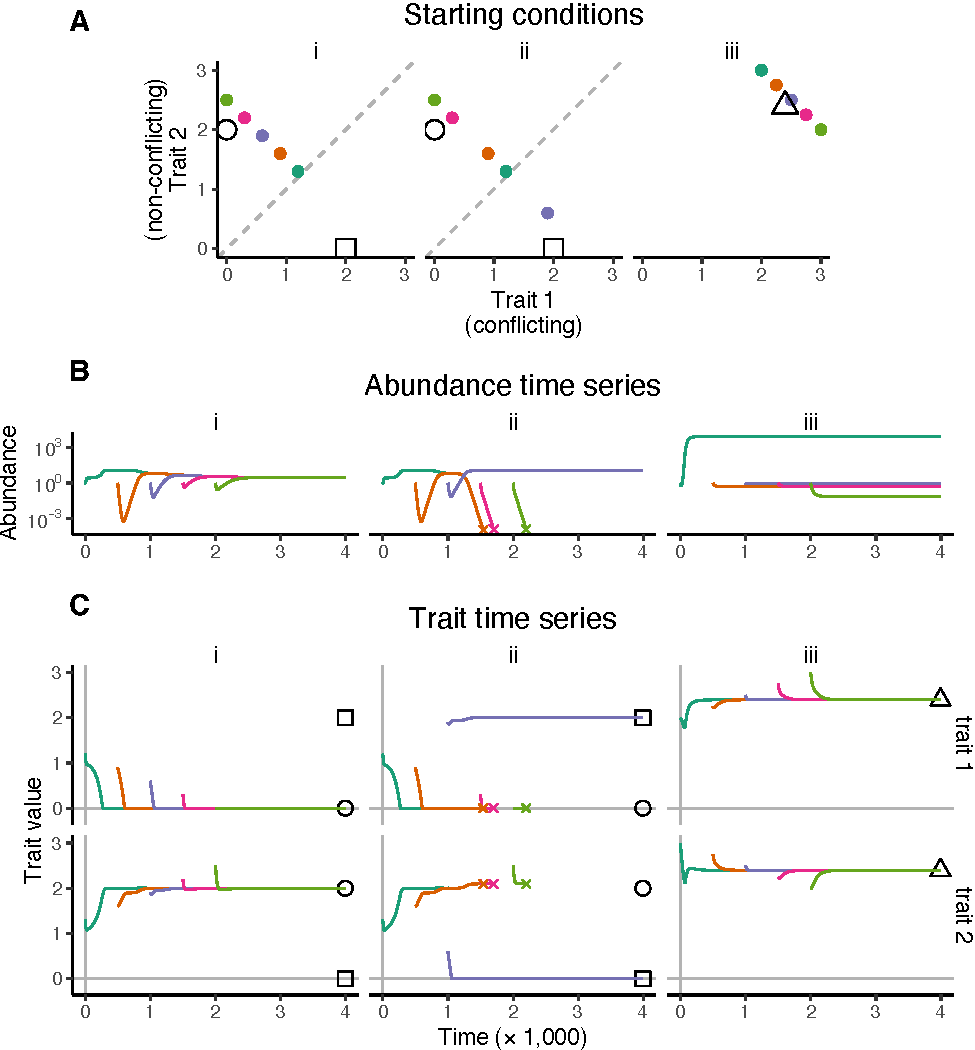
\includegraphics{3-cond_coexist_conflicting.pdf}
\caption{Conditional coexistence for 2-trait, 5-species communities when trait 1 has 
    conflicting evolution and trait 2 has non-conflicting.
    Panels show, for each of three situations,
    (A) starting conditions for each species in trait space, 
    (B) abundances through time, and 
    (C) trait values through time.
    Situations i and ii have super-additive tradeoffs, while situation iii has 
    sub-additive.
    In (A), the dotted line separates the basins of attraction for the two possible
    trait states.
    In (A,C), shapes of hollow points indicate the equilibrium trait state.
    In (B,C), Xs mark extinction events.
}
\label{fig:conditional-coexistence}
\end{figure}










Super-additivity can lead to multiple possible trait states in a 
community.
When species start with trait values that vary widely 
across the trait space, both trait states can be occupied 
simultaneously only when evolution for both traits is non-conflicting.
However, when one trait is non-conflicting and all starting
trait values in the community lie in the basin of attraction
for that trait being maximized, then coexistence can occur
(Figure \ref{fig:cond-coexist}).
Thus, even in this simple case, community evolution can follow
one of two paths depending on starting conditions:
One species evolves fastest to the conflicting state and 
excludes others, or
multiple species evolve to the non-conflicting state
and coexist.

